\hypertarget{standardSlipSystem_8cpp}{\section{standard\-Slip\-System.\-cpp \-File \-Reference}
\label{d8/d92/standardSlipSystem_8cpp}\index{standard\-Slip\-System.\-cpp@{standard\-Slip\-System.\-cpp}}
}


\-Definition of the member functions of the \hyperlink{classStandardSlipSystem}{\-Standard\-Slip\-System} class.  


{\ttfamily \#include \char`\"{}standard\-Slip\-System.\-h\char`\"{}}\*
\-Include dependency graph for standard\-Slip\-System.\-cpp\-:\nopagebreak
\begin{figure}[H]
\begin{center}
\leavevmode
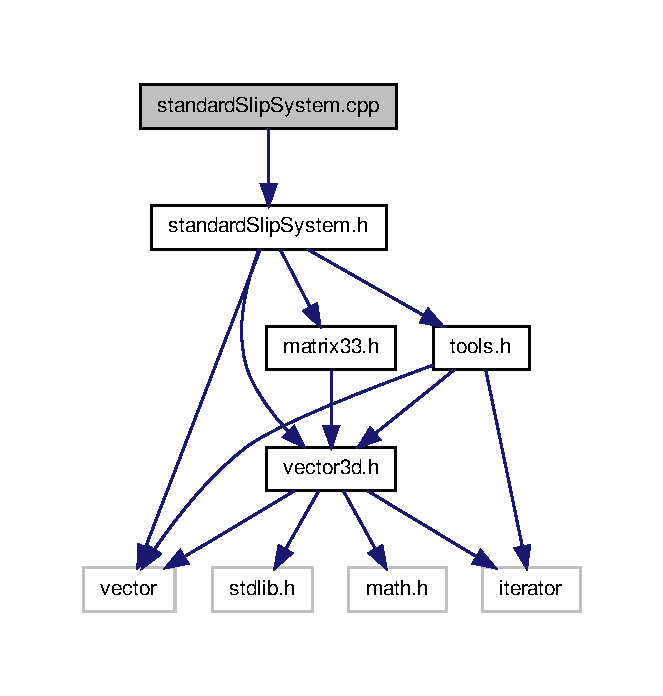
\includegraphics[width=318pt]{d4/dbc/standardSlipSystem_8cpp__incl}
\end{center}
\end{figure}


\subsection{\-Detailed \-Description}
\-Definition of the member functions of the \hyperlink{classStandardSlipSystem}{\-Standard\-Slip\-System} class. \begin{DoxyAuthor}{\-Author}
\-Adhish \-Majumdar 
\end{DoxyAuthor}
\begin{DoxyVersion}{\-Version}
0.\-0 
\end{DoxyVersion}
\begin{DoxyDate}{\-Date}
07/06/2013
\end{DoxyDate}
\-This file defines the member functions of the \hyperlink{classStandardSlipSystem}{\-Standard\-Slip\-System} class representing a slip system in the simulation. \-This class will basically be used to store the various possible slip systems corresponding different crystal structures. 

\-Definition in file \hyperlink{standardSlipSystem_8cpp_source}{standard\-Slip\-System.\-cpp}.

